% Paquets généraux
\documentclass[a4paper,12pt,titlepage,twoside]{article}
\usepackage[utf8]{inputenc}
\usepackage[T1]{fontenc}
\usepackage[french]{babel}
\usepackage{textgreek}
\usepackage[gen]{eurosym}
%\usepackage[dvips]{graphicx}
\usepackage{fancyhdr}
\usepackage{pdfpages}
\usepackage{multido}
\usepackage{hyperref}
\usepackage{numprint}
\nplpadding{2}
\usepackage{pstricks}
%\usepackage{aeguill}

\newcommand{\id}{54}
\newcommand{\nom}{Liaisons mécaniques}
\newcommand{\sequence}{04}
\newcommand{\num}{01}
\newcommand{\type}{TP}
\newcommand{\descrip}{Modélisation d'un solide. Comportement des liaisons mécaniques. Modéliser les mécanismes du laboratoire par un schéma cinématique, paramétré.}
\newcommand{\competences}{A3-C4: Analyse d'architecture et de comportement \\ &  Mod1-C1: Isolement d'un solide ou d'un système de solides \\ &  Mod2-C10-1: Modèle de solide indéformable \\ &  Mod2-C11: Modélisation géométrique et cinématique des mouvements entre solides indéformables \\ &  Mod2-C12: Modélisation cinématique des liaisons entre solides \\ &  Mod2-C15: Modélisation des actions mécaniques \\ &  Rés-C6: Utilisation d'un solveur ou d'un logiciel multi physique \\ &  Com1-C1: Différents descripteurs introduits dans le programme \\ &  Com2-C4: Outils de communication}
\newcommand{\nbcomp}{9}
\newcommand{\systemes}{Plateforme Stewart}
\newcommand{\systemessansaccent}{Plateforme Stewart}
\newcommand{\ilot}{2}
\newcommand{\ilotstr}{02}
\newcommand{\dossierilot}{\detokenize{Ilot_02 Plateforme Stewart}}
\newcommand{\imageun}{Plateforme}

\newcommand{\urlsysteme}{\href{https://www.costadoat.fr/systeme/57}{Ressources système}}
\newcommand{\matlabsimscape}{\href{https://github.com/Costadoat/Sciences-Ingenieur/raw/master/Systemes/Plateforme Stewart/Plateforme_Stewart_Simscape.zip}{Modèle Simscape}}
\newcommand{\solidworks}{\href{https://github.com/Costadoat/Sciences-Ingenieur/raw/master/Systemes/Plateforme Stewart/Plateforme_Stewart_Solidworks.zip}{Modèle Solidworks}}
\newcommand{\edrawings}{\href{https://github.com/Costadoat/Sciences-Ingenieur/raw/master/Systemes/Plateforme Stewart/Plateforme_Stewart.EASM}{Modèle eDrawings}}
\newcommand{\test}{Stewart_param1}
\newcommand{\testi}{Stewart_param2}
\newcommand{\testii}{Stewart_param3}
\newcommand{\testiii}{Stewart_param4}
\newcommand{\testiiii}{Stewart_euler}

\newcommand\twodigits[1]{%
   \ifnum#1<10 0#1\else #1\fi
}

\newcommand{\auteurun}{Renaud Costadoat}
\newcommand{\auteurdeux}{Françoise Puig}
\newcommand{\auteurs}{Costadoat - Puig}
\newcommand{\institute}{Lycée Dorian}
\newcommand{\scriptpython}{\href{https://raw.githubusercontent.com/Costadoat/S\sequence/master/\type\num\space\nom/Ilot_\twodigits{\ilot} \systemes/\sequence-\type\num-I\twodigits{\ilot}.py}{script python }}

\usepackage{color}
\usepackage{xcolor}
\usepackage{colortbl}
\usepackage{helvet}
\renewcommand{\familydefault}{\sfdefault}
\usepackage{amsfonts}
\usepackage{amsmath}
%\usepackage{xspace}
\usepackage{varioref}
\usepackage{tabularx}
%\usepackage{floatflt}
\usepackage{graphics}
\usepackage{wrapfig}
\usepackage{textcomp}
\usepackage{tikz}
\usepackage{wrapfig}
\usepackage{gensymb}
\usepackage[european]{circuitikz}
\usetikzlibrary{babel}
\usepackage{ifthen}
\usepackage{cancel}
\usepackage{etoolbox}
\usepackage{multirow}
%\usepackage{boxedminipage}
\definecolor{gris25}{gray}{0.75}
\definecolor{analyser}{RGB}{196,189,151}
\definecolor{analyserf}{RGB}{73,69,41}
\definecolor{modeliser}{RGB}{252,213,180}
\definecolor{modeliserf}{RGB}{226,107,10}
\definecolor{resoudre}{RGB}{216,228,188}
\definecolor{resoudref}{RGB}{118,147,60}
\definecolor{experimenter}{RGB}{230,184,183}
\definecolor{experimenterf}{RGB}{150,54,52}
\definecolor{concevoir}{RGB}{141,180,226}
\definecolor{concevoirf}{RGB}{15,36,62}
\definecolor{realiser}{RGB}{184,204,228}
\definecolor{realiserf}{RGB}{54,96,146}
\definecolor{communiquer}{RGB}{204,192,218}
\definecolor{communiquerf}{RGB}{96,73,122	}
\definecolor{bleu}{RGB}{18,33,98}
\definecolor{bleutf}{RGB}{8,53,154}
\definecolor{bleuf}{RGB}{42,94,171}
\definecolor{bleuc}{RGB}{231,239,247}
\definecolor{rougef}{RGB}{185,18,27}
\definecolor{rougec}{RGB}{255,188,204}%255,230,231
\definecolor{vertf}{RGB}{103,126,82}
\definecolor{vertc}{RGB}{220,255,191}
\definecolor{forestgreen}{rgb}{0.13,0.54,0.13}
\definecolor{blcr}{rgb}{0.59,0.69,0.84}
\definecolor{blfr}{rgb}{0.32,0.51,0.75}
\definecolor{orfr}{rgb}{0.90,0.42,0.15}
\definecolor{orcr}{rgb}{0.90,0.65,0.50}
\definecolor{orangef}{rgb}{0.89,0.56,0.16}
\definecolor{orange}{rgb}{0.58,0.35,0.063}
\definecolor{orangec}{rgb}{0.94,0.76,0.56}
\definecolor{rcorrect}{rgb}{0.6,0,0}
\definecolor{sequence}{rgb}{0.75,0.75,0.75}
\definecolor{competences}{rgb}{0.61,0.73,0.35}
\definecolor{grisf}{HTML}{222222}
\definecolor{grisc}{HTML}{636363}
\definecolor{normal}{HTML}{4087c4}
\definecolor{info}{HTML}{5bc0de}
\definecolor{success}{RGB}{92,184,92}
\definecolor{warning}{RGB}{240,173,78}
\definecolor{danger}{RGB}{217,83,79}
\hypersetup{                    % parametrage des hyperliens
    colorlinks=true,                % colorise les liens
    breaklinks=true,                % permet les retours à la ligne pour les liens trop longs
    urlcolor= blfr,                 % couleur des hyperliens
    linkcolor= orange,                % couleur des liens internes aux documents (index, figures, tableaux, equations,...)
    citecolor= forestgreen                % couleur des liens vers les references bibliographiques
    }

% Mise en page
\pagestyle{fancy}

\setlength{\hoffset}{-18pt}

\setlength{\oddsidemargin}{0pt} 	% Marge gauche sur pages impaire2s
\setlength{\evensidemargin}{0pt} 	% Marge gauche sur pages paires
\setlength{\marginparwidth}{00pt} 	% Largeur de note dans la marge
\setlength{\headwidth}{481pt} 	 	% Largeur de la zone de tête (17cm)
\setlength{\textwidth}{481pt} 	 	% Largeu\textbf{r de la zone de texte (17cm)
\setlength{\voffset}{-18pt} 		% Bon pour DOS
\setlength{\marginparsep}{7pt}	 	% Séparation de la marge
\setlength{\topmargin}{-30pt} 		% Pas de marge en haut
\setlength{\headheight}{45pt} 		% Haut de page
\setlength{\headsep}{20pt} 			% Entre le haut de page et le texte
\setlength{\footskip}{30pt} 		% Bas de\textbf{ page + séparation
\setlength{\textheight}{700pt} 		% Hauteur de l'icone zone de texte (25cm)
\setlength\fboxrule{1 pt}
\renewcommand{\baselinestretch}{1}
\setcounter{tocdepth}{1}
\newcommand{\cadre}[2]
{\fbox{
  \begin{minipage}{#1\linewidth}
   \begin{center}
    #2\\
   \end{center}
  \end{minipage}
 }
}

\newcounter{num_quest} \setcounter{num_quest}{0}
\newcounter{num_rep} \setcounter{num_rep}{0}
\newcounter{num_cor} \setcounter{num_cor}{0}

\newcommand{\question}[1]{\refstepcounter{num_quest}\par
~\ \\ \parbox[t][][t]{0.15\linewidth}{\textbf{Question \arabic{num_quest}}}\parbox[t][][t]{0.93\linewidth}{#1}\par
}


\newcommand{\reponse}[1]
{\refstepcounter{num_rep}
\noindent
\rule{\linewidth}{.5pt}
\textbf{Question \arabic{num_rep}:}
\multido{\i=1+1}{#1}{~\ \\}
}

\newcommand{\cor}
{\refstepcounter{num_cor}
\noindent
\rule{\linewidth}{.5pt}
\textbf{Question \arabic{num_cor}:} \\
}

\newcommand{\titre}[1]
{\begin{center}
\cadre{0.8}{\huge #1}
\end{center}
}

%Titres des sections

\newcommand{\titleana}[2]{%
\tikzstyle{titlebox}=[rectangle,inner sep=10pt,inner ysep=10pt,draw,fill=analyser]%
\tikzstyle{title}=[fill=analyser]%
%
\bigskip\noindent\begin{tikzpicture}
\node[titlebox] (box){%
\begin{minipage}{0.94\textwidth}
\textbf{\textcolor{analyserf}{#1}}
\end{minipage}
};
%\draw[color=blue] (box.north west)--(box.north east);
\node[title] at (box.north) {\textcolor{analyserf}{ANALYSER}};
\end{tikzpicture}%
\\}

\newcommand{\titlemod}[2]{%
\tikzstyle{titlebox}=[rectangle,inner sep=10pt,inner ysep=10pt,draw,fill=modeliser]%
\tikzstyle{title}=[fill=modeliser]%
%
\bigskip\noindent\begin{tikzpicture}
\node[titlebox] (box){%
\begin{minipage}{0.94\textwidth}
\textbf{\textcolor{modeliserf}{#1}}
\end{minipage}
};
%\draw[color=blue] (box.north west)--(box.north east);
\node[title] at (box.north) {\textcolor{modeliserf}{MODELISER}};
\end{tikzpicture}%
\\}

\newcommand{\titleres}[2]{%
\tikzstyle{titlebox}=[rectangle,inner sep=10pt,inner ysep=10pt,draw,fill=resoudre]%
\tikzstyle{title}=[fill=resoudre]%
%
\bigskip\noindent\begin{tikzpicture}
\node[titlebox] (box){%
\begin{minipage}{0.94\textwidth}
\textbf{\textcolor{resoudref}{#1}}
\end{minipage}
};
%\draw[color=blue] (box.north west)--(box.north east);
\node[title] at (box.north) {\textcolor{resoudref}{RESOUDRE}};
\end{tikzpicture}%
\\}

\newcommand{\titleexp}[2]{%
\tikzstyle{titlebox}=[rectangle,inner sep=10pt,inner ysep=10pt,draw,fill=experimenter]%
\tikzstyle{title}=[fill=experimenter]%
%
\bigskip\noindent\begin{tikzpicture}
\node[titlebox] (box){%
\begin{minipage}{0.94\textwidth}
\textbf{\textcolor{experimenterf}{#1}}
\end{minipage}
};
%\draw[color=blue] (box.north west)--(box.north east);
\node[title] at (box.north) {\textcolor{experimenterf}{EXPERIMENTER}};
\end{tikzpicture}%
\\}

\newcommand{\titlecon}[2]{%
\tikzstyle{titlebox}=[rectangle,inner sep=10pt,inner ysep=10pt,draw,fill=concevoir]%
\tikzstyle{title}=[fill=concevoir]%
%
\bigskip\noindent\begin{tikzpicture}
\node[titlebox] (box){%
\begin{minipage}{0.94\textwidth}
\textbf{\textcolor{concevoirf}{#1}}
\end{minipage}
};
%\draw[color=blue] (box.north west)--(box.north east);
\node[title] at (box.north) {\textcolor{concevoirf}{CONCEVOIR}};
\end{tikzpicture}%
\\}

\newcommand{\titlerea}[2]{%
\tikzstyle{titlebox}=[rectangle,inner sep=10pt,inner ysep=10pt,draw,fill=realiser]%
\tikzstyle{title}=[fill=realiser]%
%
\bigskip\noindent\begin{tikzpicture}
\node[titlebox] (box){%
\begin{minipage}{0.94\textwidth}
\textbf{\textcolor{realiserf}{#1}}
\end{minipage}
};
%\draw[color=blue] (box.north west)--(box.north east);
\node[title] at (box.north) {\textcolor{realiserf}{REALISER}};
\end{tikzpicture}%
\\}

\newcommand{\titlecom}[2]{%
\tikzstyle{titlebox}=[rectangle,inner sep=10pt,inner ysep=10pt,draw,fill=communiquer]%
\tikzstyle{title}=[fill=communiquer]%
%
\bigskip\noindent\begin{tikzpicture}
\node[titlebox] (box){%
\begin{minipage}{0.94\textwidth}
\textbf{\textcolor{communiquerf}{#1}}
\end{minipage}
};
%\draw[color=blue] (box.north west)--(box.north east);
\node[title] at (box.north) {\textcolor{communiquerf}{COMMUNIQUER}};
\end{tikzpicture}%
\\}


\newcommand{\prob}[2]{%
\tikzstyle{titlebox}=[rounded corners=10,inner sep=10pt,inner ysep=10pt,draw,fill=bleuf]%
%\tikzstyle{title}=[]%
%
\bigskip\noindent\begin{tikzpicture}
\node[titlebox] (box){%
\begin{minipage}{0.94\textwidth}
\begin{minipage}{0.15\linewidth}

\includegraphics[width=0.8\linewidth]{../../../img/questionmark}
\end{minipage}
\begin{minipage}{0.8\linewidth}
\textbf{\textcolor{white}{
 Problématique du TP:\\ \noindent\rule{13cm}{1pt} \\ \\#1}}
\end{minipage}
\end{minipage}
};
%\draw[color=blue] (box.north west)--(box.north east);
%\node[title] at (box.north west) {\textcolor{white}{\textbf{Problématique}}};
\end{tikzpicture}\bigskip\\~\ \\%
}

%Procédures logiciels

\newcommand{\proceduresimscape}{
\begin{center}
 \huge{Utilisation de Matlab Simscape}
\end{center}

La procédure suivante explique comment utiliser Matlab afin de simuler un modèle Simscape.

Ce modèle a été construit à partir des pièces, assemblages et contraintes d'un modèle Solidworks. Ce dernier n'est pourtant pas nécessaire pour le faire tourner.

\medskip

Procédure :
\begin{itemize}
 \item Dézipper l'archive à télécharger ici \matlabsimscape,
 \item Lancer Matlab 
\includegraphics[width=80pt]{../../../img/matlabsimscape/matlab}
 \item Depuis Matlab, naviguer 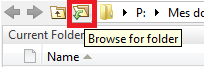
\includegraphics[width=80pt]{../../../img/matlabsimscape/matlab_01} dans le dossier dézippé jusqu'au dossier contenant les fichiers \og .slx \fg\ et \og Simscape \fg,\\
  \begin{center}
  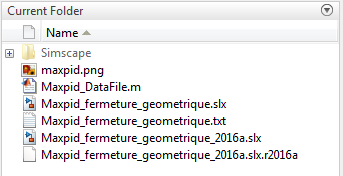
\includegraphics[width=0.4\linewidth]{../../../img/matlabsimscape/matlab_02}
  \end{center}
 \item Faire un clic-droit sur le dossier \og Simscape \fg\ et cliquer sur \og Add to Path \fg,\\
  \begin{center}
  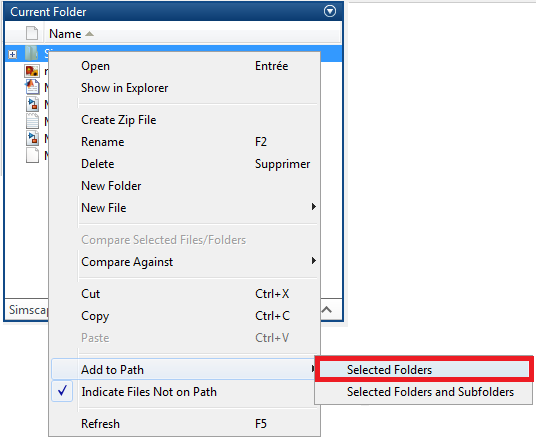
\includegraphics[width=0.4\linewidth]{../../../img/matlabsimscape/matlab_03}
  \end{center}
 \item Double-cliquer sur le fichier correspondant au TP et à la version de Matlab utilisée, il doit avoir une extension en \og slx \fg.\\
  \begin{center}
  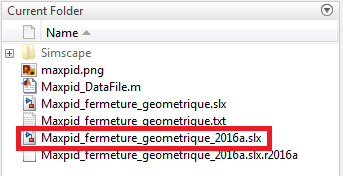
\includegraphics[width=0.4\linewidth]{../../../img/matlabsimscape/matlab_04}
  \end{center}
\end{itemize}
}























% En tête et pied de page
\lhead{\nom}
\rhead{
\includegraphics[width=2cm]{../../../img/logo}}
\lfoot{\auteurs}
\cfoot{Page \thepage}

\fancypagestyle{correction}{%
  \fancyhf{}
  \lhead{\colorbox{danger}{\begin{minipage}{0.65\paperwidth} \textcolor{white}{\textbf{Correction}} \end{minipage}} }
  \rhead{
\includegraphics[width=2cm]{../../../img/logo}}
  \lfoot{Renaud Costadoat}
  \rfoot{\colorbox{danger}{\begin{minipage}{0.6\paperwidth} \begin{flushright}\textcolor{white}{\textbf{Correction}}\end{flushright} \end{minipage}} }}

\renewcommand{\footrulewidth}{0.4pt}

\usepackage{eso-pic}
\newcommand{\BackgroundPic}{%
\put(0,0){%
\parbox[b][\paperheight]{\paperwidth}{%
\vfill
\begin{center}
\hspace{0.5cm}\vspace{0.5cm}

\includegraphics[width=\paperwidth,height=\paperheight,%
keepaspectratio]{../../../img/fond3}%
\end{center}
\vfill
}}}

\newcommand{\BackgroundPicdeux}{%
\put(25,-30){%
\parbox[b][\paperheight]{\paperwidth}{%
\vfill
\begin{center}

\includegraphics[width=\paperwidth,height=\paperheight,%
keepaspectratio]{../../../img/fond4}%
\end{center}
\vfill
}}}

\newcommand{\activite}[1]{\newpage \cleardoublepage
\renewcommand\arraystretch{2.5}\setcounter{section}{0}\setcounter{subsection}{0}
\ifthenelse{\equal{#1}{1}}{\begin{center}\begin{tabular}{|c|cc p{3cm}|}
\hline
\rowcolor{violt} \supportu & Act & Contenu & Compétences \\\hline
 \multirow{3}{*}{\includegraphics[width=0.2\linewidth]{\supportimageu}} & \begin{LARGE}\textbf{1}\end{LARGE} & \activiteun & \competenceun \\
 & \multicolumn{3}{l|}{Nom: .........................................................................}\\
 & \multicolumn{3}{l|}{Prénom: ....................................................................}\\\hline
\end{tabular}\end{center}}{}
\ifthenelse{\equal{#1}{2}}{\begin{center}\begin{tabular}{|c|cc p{3cm}|}
\hline
\end{tabular}\end{center}}{}}

\begin{document}

\pagestyle{empty}

\vspace*{-3\baselineskip}

\AddToShipoutPicture*{\BackgroundPic}

\ifdef{\auteurdeux}{\begin{tabular}{>{\columncolor{gray!00}}m{.33\linewidth} m{.27\linewidth} >{\columncolor{gray!00}}m{.3\linewidth}}
Séquence \sequence \ - \type \num \ - Îlot \numprint{\ilot} &  \multirow{3}{*}{\hspace{1cm}
\includegraphics[height=1.5cm]{../../../img/logo}} &  \begin{flushright} \multirow{4}{*}{\hspace{1cm}
\includegraphics[height=4cm]{img/qrcode}}\end{flushright}\\
 \textbf{\institute} \\
 \auteurun\\
 \auteurdeux
\end{tabular}}{\begin{tabular}{>{\columncolor{gray!00}}m{.3\linewidth} m{.3\linewidth} >{\columncolor{gray!00}}m{.3\linewidth}}
Séquence \sequence \ - \type \num \ - Îlot \numprint{\ilot}  &  \multirow{3}{*}{\hspace{1cm}
\includegraphics[height=1.5cm]{../../../img/logo}} &  \begin{flushright} \multirow{4}{*}{\hspace{1cm}
\includegraphics[height=4cm]{img/qrcode}}\end{flushright}\\
 \textbf{\institute} \\
 \auteurun
\end{tabular}}

\vspace{1cm}

\begin{center}\colorbox{white}{\huge{\nom}}\end{center}

\vspace{2cm}


\begin{center}\colorbox{white!20}{\includegraphics[height=5cm]{/home/renaud/Documents/Renaud/GitHub/django_education/django_education/static/systemes/\imageun}}\end{center}

\vspace{2cm}



\begin{tabular}{p{.15\linewidth} >{\columncolor{white}}p{.8\linewidth}}
    \rowcolor{gray!20}
    Référence & S\sequence \ - \type\num \ - I\numprint{\ilot} \\
    Compétences & \competences \\
 	\rowcolor{gray!20}
    Description & \descrip \\
    Système & \systemes
  \end{tabular}

\newpage

\AddToShipoutPicture{\BackgroundPicdeux}

\pagestyle{fancy}


\prob{Analyse et mise en \oe uvre d'un système} 

Remarque: Les réponses aux questions suivantes devront, à chaque fois que c'est possible, être mises sous la forme de diagramme SysMl.

\titleana{Déterminer la fonction globale du système} 

La Diravi est une direction assistée installée sur une Citroën CX.

\paragraph{Question 1:} Donnerez la ou les principale(s) fonction(s) du système \og Diravi \fg. De ces fonctions découlent des exigences, en proposer au moins trois. A ces exigences devront être associés des niveaux qui permettent de les classer par ordre d'importance.

\paragraph{Question 2:} A quel(s) acteur(s) ce système rend-il service ? Comment celui-ci(ceux-ci) se rend(ent)-il(s) compte du service rendu ?

\titleexp{Montrer que le système répond au cahier des charges}

\paragraph{Question 3:} Effectuer une rotation complète du volant sans mettre en service la pompe puis en mettant la pompe en service. Constater l'influence de l'assistance sur l'action du conducteur sur le volant.

\paragraph{Question 4:} Faire varier la vitesse du véhicule grâce au potentiomètre et montrer l'influence de la vitesse du l'assistance.

\paragraph{Question 5:} Proposer un protocole expérimental permettant de déterminer l'action exercée par le conducteur avec et sans assistance.

\titleana{Éléments du Milieu Extérieur}

Lors de la phase de vie du système correspondant à son \og utilisation \fg, celui-ci se trouve intégré à une voiture.

\paragraph{Question 6:} A quels éléments extérieurs liés à l'environnement la diravi est-elle confrontée lors de cette phase de vie ? Ces éléments ont-ils été pris en compte lors de l'étude de la conception de la diravi ? Comment ?

\paragraph{Question 7:} A quelles sources d'énergie la diravi doit-elle être connectée afin de fonctionner correctement ?

\paragraph{Question 8:} Proposez des solutions qui d'après vous ont été appliqués au système afin d'assurer la sécurité des utilisateur et de l'installation.

\paragraph{Question 9:} En considérant l'ilot comme étant tout ce qui se trouve sur la table (en dehors de vos affaires) quels sont les éléments qui ne font pas partie du système diravi ? Celui-ci fonctionnerait-il sans leur présence ?

\titleana{Composants du système}

Le système diravi est constitué de plusieurs sous-systèmes qui participent à la réalisation des actions attendues de la diravi.

\paragraph{Question 10:} Donner le nom d'un certain nombre de sous-systèmes qui composent la diravi. Pour chacun de ces sous-systèmes, vous préciserez s'ils sont ou non obligatoires pour le bon fonctionnement du système ou s'ils sont facultatifs.

\paragraph{Question 11:} Ces blocs devront ensuite être classés, si possible, dans une des familles suivantes:
\begin{itemize}
 \item système de calcul,
 \item capteur,
 \item effecteur (moteur, vérin,...),
 \item système mécanique,
 \item carter/protection,
 \item système de communication,
 \item alimentation,
 \item ...
\end{itemize}

\titlemod{Flux traversants}

Les blocs qui ont été trouvés précédemment sont reliés entre eux par des flux :
\begin{itemize}
 \item d'énergie,
 \item de matière,
 \item d'information
\end{itemize}

\paragraph{Question 12:} Donner l'ensemble des flux qui entrent dans la diravi et ceux qui en sortent. Ces flux devront être classés selon les trois catégories décrites précédemment.

Chaque flux entrant/sortant transite pour entrer/sortir du système par un port.

\paragraph{Question 13:} Donner pour chaque flux le port par lequel il transite. Ces ports sont-ils unidirectionnel ou bien servent-ils à faire à la fois entrée et sortir un flux ?

\paragraph{Question 14:} Les flux énergétiques doivent être classés en fonction du type d'énergie qui transite:
\begin{itemize}
 \item électrique,
 \item mécanique de translation,
 \item mécanique de rotation,
 \item thermique,
 \item ...
\end{itemize}

\titleexp{Mise en \oe uvre du système}

Mettre en \oe uvre le système et effectuer une mesure.

\paragraph{Question 15:} Décrire succinctement (mais précisément) les opérations à effectuer par l'utilisateur durant cette mise en \oe uvre ainsi que les messages que le système envoie à l'utilisateur.

\paragraph{Question 16:} Décrire succinctement (mais précisément) le comportement du système. Donner notamment:
\begin{itemize}
 \item l'état initial,
 \item l'état final,
 \item les actions effectuées par le système,
 \item ...
\end{itemize}

\titleexp{Déterminer de l'état du système}

La partie qui pilote le système doit connaître son état afin d'agir en conséquence. 

\paragraph{Question 17:} Donner l'ensemble des éléments qui permettent à la partie commande de récupérer des informations sur l'état du système.

\paragraph{Question 18:} Pour chacun de ces éléments, vous donnerez le type d'information qu'il est capable de capter/détecter.

\titleana{Chaînes d'énergie et d'information}

Comme tout système automatisé, la diravi peut être décrit sous la forme de chaînes d'information et d'énergie.

\paragraph{Question 19:} En utilisant les résultats des activités précédentes, vous complèterez les chaînes d'énergie et d'information fournies dans le document de présentation.

La diravi a été conçue en répondant aux exigences issues d'un cahier des charges, rédigé par le concepteur en collaboration avec le client. Le concepteur a ensuite dû trouver des solutions techniques afin de répondre aux exigences 

\paragraph{Question 20:} En utilisant les résultats des activités précédentes, trouver les solutions techniques qui ont permis de répondre aux exigences du cahier des charges.

\titlecom{Synthèse du travail de groupe}

\paragraph{Question 21:} Préparer une présentation (10 min) à partir du document de présentation complété pendant le TP. Répartir le temps de parole entre les intervenant et veiller à faire respecter (cordialement) ce temps de parole. Il est recommandé de ne pas lire de fiche pendant la présentation et de s'appuyer sur le \og Document ressources \fg établit durant la séance. Ce document pourra être complété comme vous le souhaitez.

~\

La présentation doit se dérouler de la manière suivante:
\begin{itemize}
 \item Introduction (resp 4),
 \begin{itemize}
 \item Présentation du système,
 \item Présentation du travail des membres du groupe.
 \end{itemize}
 \item Passage des membres du groupe
 \item Conclusion (resp 4),
 \begin{itemize}
 \item Conclusion sur le travail effectué,
 \item Conclusion sur l'intérêt du système.
 \end{itemize}
\end{itemize}



\end{document}
